% !TeX root = ../../main.tex

\section{Background and Motivation}

\emph{Bulk synchronous parallel} (BSP)~\cite{Valia1990:BSP} workloads in both scientific computing and machine learning
training pose unique efficiency challenges.
These jobs, increasingly spanning tens of thousands of nodes, execute in lockstep and synchronize
frequently via collective communication.
At these scales, BSP is uniquely fragile: a single straggler can block cluster-wide progress at
synchronization points.
% \cite{Petri2003:Missing,VanS2009:AMR,Kocol2018:Varbench,Gunaw2018:FailSlow,Acun2016:Mitigating,Acun2016:Variation,Lu2023:PERSEUS,Yildi2016:IONoise,You2024:GVARP,Xuan2025:IdentifyingPerformanceInefficiencies,Gangi2024:RDMA,Jain2025:AMR}
Their root causes are highly context-dependent, ranging from load imbalance and suboptimal overlap
to tuning-induced variability, and have been documented
extensively~\cite{Petri2003:Missing,VanS2009:AMR,Kocol2018:Varbench,Gunaw2018:FailSlow,Acun2016:Mitigating,Acun2016:Variation,Lu2023:PERSEUS,Yildi2016:IONoise,You2024:GVARP,Xuan2025:STAD,Gangi2024:RDMA,Jain2025:AMR}.
Despite extensive studies, general-purpose mechanisms for operational visibility into BSP
application performance remain elusive.
% Despite this, principled ways to obtain actionable visibility into application performance in
% production HPC environments remain elusive.


% \subsection{Motivation: Closing the Feedback Loop}

% Whereas monitoring targets \emph{known unknowns} via a fixed set of metrics such as CPU and memory
% utilization, performance pathologies in BSP workloads are dominated by \emph{unknown unknowns}.
% Observability~\cite{Major2017:o11y,Major2020:o11y,:OtelO11y,Sridh:DistributedSystemsObservability}
% in this context is the ability to resolve them by constructing the right views from telemetry and
% refining them until causal attribution is possible.

% Dominant observability paradigms for BSP workloads make this loop slow and rare.
% Diagnosing pathologies requires rerunning applications under progressively heavier diagnostics,
% from lightweight aggregates collected as profiles to fine-grained traces captured as per-rank event
% logs.
% At scale, these traces are too large to inspect visually, and programmatic analyses require
% expensive \emph{extract-transform-load} (ETL)~\cite{Yildi2023:IOMax} before queries can be served.
% % Identifying anomalies within traces either requires visual inspection, impractical beyond modest
% % scales, or programmatic analyses, which require expensive extract-transform-load (ETL) stages.
% Additional instrumentation or interventions require repeating this workflow multiple times to
% isolate root causes and verify fixes.
% As a result, operators are forced to choose between expensive investigations and ad-hoc
% workarounds.

% This gap motivates a different model: always-on observability as an operational capability, with
% relevant views derived in real-time, hypotheses tested live, and collection steered accordingly
% while the job is still running.

% \subsection{Case Studies from HPC and ML}
% \subsubsection{Optimizing Placement in AMR}
% \figBgVolatile{}
% reproduce this differently?

% insert figure
\begin{figure}[t]
  \centering
  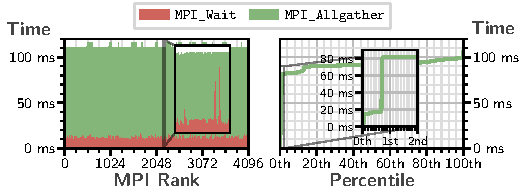
\includegraphics[width=\columnwidth]{data/figs/orca_lesson_volfunc_single_cdf.pdf}
  \caption{Telemetry from \Cref{fig:amr:chal:vol} showing volatile \mpiw{} preceding \texttt{MPI\_Allgather}.\\
  (Left) Identifying stragglers requires fine-grained per-rank telemetry joined by timestep.\\
  (Right) Percentiles over per-timestep collective durations can be converted into lightweight metrics for continuous monitoring. Here, 1\textsuperscript{st}-percentile collective durations would reveal stragglers.}
  \label{fig:orca:bg-volatile}
\end{figure}

% \cite{Jain2025:AMR}
% \cite{Dubey2014:Survey} (AMR load-imbalance challenges)
% Our study of placement and load-balancing in \emph{adaptive mesh refinement} (AMR)
% codes~\cite{Jain2025:AMR} illustrates this gap concretely.
% While widely known for load-imbalance challenges~\cite{Dubey2014:Survey}, we found that genuine
% load-imbalance was indistinguishable from other hardware, software, and tuning artifacts without
% fine-grained telemetry.
% \Cref{fig:orca:bg-volatile} shows one such example: tail latency spikes in \mpiw{}
% that only manifested at scale would get attributed to collectives in aggregate telemetry.
% Each artifact took us months of iterative diagnoses, while mitigations would typically only take a
% few days.

% Diagnosing each of theses issues required multiple iterations of fine-grained capture and ETL-heavy
% analysis over formats such as CSV.
% The mitigations identified were specific to our cluster and workload.
% Even after these artifacts were fixed, our placement policies demonstrated a fundamental tradeoff
% between compute load balance and communication locality --- the right balance between the two
% varies across workloads, scales, and architectures.
% Translating these optimizations to production environments would require repeating this
% time-consuming exercise --- underscoring the need for infrastructure that makes such investigations
% routine.
% Translating them to production environments would require repeating the same exercise.
% Given that optimal configurations are not portable across environments, the need is not for better
% one-off analyses but for infrastructure that makes such investigations routine.

\subsection{Parallels from the Pytorch Ecosystem}

% \cite{2025:PytorchKineto} (Kineto)
% \cite{2025:MetaDynolog} (Dynolog)
% \cite{2025:MetaHTA} (HTA)
The PyTorch~\cite{Paszk2019:PyTorch} ecosystem exhibits the same pattern.
Kineto~\cite{2025:PytorchKineto} captures fine-grained traces on demand as JSON.
Dynolog~\cite{2025:MetaDynolog} provides node-local control to trigger capture.
\emph{Holistic Trace Analysis} (HTA)~\cite{2025:MetaHTA} computes derived views such as activity
breakdowns and straggler detection.
Together, these form a closed loop, but with the same shortcomings we faced in our AMR study.
HTA is a single-node Pandas~\cite{:Pandas} script that cannot scale to cluster-wide traces without
expensive ETL.
Dynolog provides best-effort actuation with no consistency guarantees, whereas reliable
construction of views like \Cref{fig:orca:bg-volatile} requires complete telemetry for each collective
instance.

The wider ML training literature reinforces this pattern.
% \cite{Yao2025:Holmes} (HOLMES: communication irregularity localization)
% \cite{Wu2025:GREYHOUND} (GREYHOUND: fail-slow detection)
% \cite{Deng2025:Minder} (Minder: faulty machine detection)
% \cite{Cui2025:XPUTimer} (XPUTimer: anomaly diagnostics)
% \cite{Dong2025:Aegis} (Aegis: failure diagnosis)
% \cite{Jiang2025:TrainCheck} (TrainCheck: numerical stability)
% \cite{Guan2025:PerfTracker}: PerfTracker
Recent systems address pathologies such as straggler
localization~\cite{Yao2025:Holmes,Wu2025:GREYHOUND,Cui2025:XPUTimer,Guan2025:PerfTracker,Deng2025:Mycroft},
fault diagnosis~\cite{Dong2025:Aegis,Deng2025:Minder}, and training
correctness~\cite{Jiang2025:TrainCheck}, but each reimplements subsets of collection, aggregation,
and control from scratch.
A common substrate would allow detection strategies to be expressed as analytics queries over
telemetry, composable and deployable without rebuilding the infrastructure beneath them.

\subsection{Existing Approaches and Gaps}

% \cite{Schwa2021:LDMS} (LDMS)
% \cite{:Prometheus} (Prometheus)
\parahead{Monitoring}
Monitoring enables basic visibility via metrics captured at sampled intervals, but lacks the
workload context for causal attribution.
Prometheus~\cite{:Prometheus} is a time-series database for system counters, while
LDMS~\cite{Schwa2021:LDMS} extends coverage for application-level statistics such as
Kokkos~\cite{Trott2022:Kokkos3}.
They can not support synchronized on-demand collection necessary for views such as
\Cref{fig:orca:bg-volatile}.

% \cite{Shend2006:TAU} (TAU)
% \cite{Knupf2012:Score-P} (Score-P)
% \cite{Eschw2012:OTF2} (OTF2)
\parahead{Profiling and Tracing}
Tools such as TAU~\cite{Shend2006:TAU}, \scorep{}~\cite{Knupf2012:Score-P}, and
Kineto~\cite{2025:PytorchKineto} can provide both high-level aggregates or fine-grained telemetry
via traces, but their workflows are post hoc by design.
Traces can characterize short runs, but cannot provide always-on visibility over long-running jobs.
In the absence of any real-time feedback to guide collection, the post hoc paradigm also
incentivizes overcollection, leading to large datasets and long delays.
Formats like OTF2~\cite{Eschw2012:OTF2} are not designed for analytics, and visual inspection for
anomalies is impractical at scale with billions of events.

% \cite{Bhate2019:Hatchet} (Hatchet)
% \cite{Yildi2023:IOMax} -- DFTracer cousin, exists because they do not know Polars + Lazy Parquet exists
\parahead{Dataframe Analytics}
Recent tools such as Caliper~\cite{Boehm2016:Caliper},
\dftracer{}~\cite{Devar2024:DFTracer}, Pipit~\cite{Bhate2024:Pipit}, and Pytorch
HTA~\cite{2025:MetaHTA} have adopted Pandas~\cite{:Pandas} and Dask-based~\cite{Rockl2015:Dask}
dataframe analytics interfaces to analyze telemetry, but require expensive
ETL~\cite{Yildi2023:IOMax} to parse entire traces written as per-rank logs in 
plaintext formats
%formats such as CSV and JSON 
--- the working set for which scales with \emph{ranks $\times$ timesteps}.
Columnar formats like Parquet~\cite{:ApacheParquet} offer efficient post-hoc analytics, but do not
by themselves address overcollection, working set scaling, or real-time feedback, and remain
largely unadopted in tracing workflows.
In a simple internal port of HTA analyses from JSON to Parquet, we observed 50$\times$ faster data loading
and 18$\times$ faster end-to-end analysis.

% \cite{Godoy2020:ADIOS2} (ADIOS)
% \cite{Eisen2024:ADIOS} -- ADIOS SST
\parahead{Streaming and In-situ Analytics}
ADIOS~\cite{Godoy2020:ADIOS2} enables fixed-function in-situ
%provides transport abstractions for in-situ
workflows~\cite{Eisen2024:ADIOS} on scientific data, typically run as another MPI application.
MRNet~\cite{Roth2003:MRNet,Willi2016:MRNetApps} is a tree-based overlay used as a reduction backend
for commercial debuggers, but provides a compiled packet-based programming model.
Neither enable runtime-programmable dataframe-style analytics needed for real-time BSP
observability.
Cloud streaming systems such as Flink~\cite{Carbo2015:ApacheFlink} and Kafka~\cite{Kreps2011:Kafka}
are designed for independent event streams over IP networks
They lack fabric-aware transport and BSP-aligned coordinated collection,
precluding views like \Cref{fig:orca:bg-volatile}.
% making them unable to guarantee the causal completeness required for views like Fig. 1.
% , not for low-jitter synchronized
% ingestion from BSP workloads.
% They can not leverage HPC fabrics or enable closed-loop BSP workflows.

\subsection{The Missing Substrate}

Diagnosing the root cause behind \Cref{fig:orca:bg-volatile} required capabilities beyond what any
single tool in the taxonomy provides.
At node scale, eBPF~\cite{:eBPF} provides a template: dynamic probes, programmatic aggregation, low
overhead in the common case with depth when needed.
It enabled controlled and targeted access to telemetry within \mpiw{} after alternatives were
exhausted.
Hypotheses about interrupts and scheduler effects were tested and discarded in hours.
But eBPF is node-local, and our workflow involved ad-hoc orchestration, uncoordinated collection,
and manual post-hoc correlation.
Extending this to workload scale---tens of thousands of BSP ranks---requires a substrate that
provides the same depth on demand, treating observability not as distributed logging, but as
constructing views directly from running applications via a programmable interface.
The next section states the requirements such a substrate must satisfy.



% ===================================
% TrainCheck: training for correctness
% ==================================

% - Defines relations on V, E, I

% V: hashes of tensors
% E: event
% I: also an event

% Consistent(Va, Vb): should have the same values.
% ORCA: timestep dataframe, groupby, distinct

% EventContain(Ea, Eb): Eb must happen within Ea
% ORCA: filter by Ea and Eb, zip or map

% APISequence: f, g, h must be called in this order
% ORCA: need a kernel

% APIArg(f, is_distinct): must be distinct if true, not if false
% ORCA: kernel

% APIOutput(f, bound_type): some constraint on output. Not described.
% ORCA: sql or kernel